\documentclass[main.tex]{subfiles}
\usepackage{svg}
\usepackage{graphicx}
\usepackage{float}
\begin{document}

This section details the Kubernetes Pod lifecycle states tested in this document and describes each transition in terms of its purpose, how it can be reached, and testing methods.

\subsection{States}
\begin{itemize}
    \item \textbf{PodNotExists}: The initial or end state when a pod is absent in the cluster. It appears before a pod is created or after it is deleted. 
    \textbf{Note:} The PodNotExists state used in this FSM model is not an actual Kubernetes Pod state. It is included solely for modeling purposes to represent when a Pod has not yet been created or has already been deleted.
    \item \textbf{Pending}: The pod is created but has not yet been scheduled onto a node, awaiting resource assignment.
    \item \textbf{ContainerCreating}: The container image is being pulled, and the pod is initializing.
    \item \textbf{ImagePullBackOff}: The pod is stuck due to an image pull error, which prevents the containers from starting.
    \item \textbf{Running\_NotReady}: The pod has started, but one or more containers are not fully ready, potentially failing readiness probes.
    \item \textbf{Running\_Ready}: The pod is fully functional with all containers running and ready, passed rediness probes.
    \item \textbf{Succeeded}: The pod has completed its task successfully, and all containers have exited without issues. It is possible only if the pod is a job, otherwise its containers won't typically exit.
    \item \textbf{Failed}: The pod has terminated due to a failure in one or more containers. 
    \item \textbf{CrashLoopBackOff}: The pod is restarting repeatedly due to a failure in one or more containers.
    \item \textbf{Terminating}: The pod is in the process of being deleted from the cluster.
\end{itemize}

\subsection{Transitions}
\subsubsection{Create Pod (PodNotExists $\rightarrow$ Pending)}
In Kubernetes, creating a Deployment is typically preferred over creating individual Pods. A Deployment defines the desired state of Pods and manages their lifecycle, ensuring that the specified number of replicas are running, handling restarts, and managing updates. When a Deployment is created, Kubernetes automatically schedules and manages the Pods to maintain the Deployment's specified state.

The user provides a YAML configuration for the Deployment, which includes metadata (e.g., name, namespace), and specification (e.g., desired replicas, Pod template with containers, images, and resources). Then the user runs \texttt{kubectl apply -f <deployment-definition>.yaml}.
\texttt{kubectl} sends a POST request (\texttt{POST /api/v1/namespaces/{namespace}/pods}) to the Kubernetes API Server with the Deployment specification. The API server validates the YAML configuration, checking for required fields (such as metadata and Pod template).
The API ensures that resource quotas, namespace permissions, and other requirements are met. The API server records the Deployment in etcd, marking the desired number of replicas.
The Deployment controller in the control plane reads the Deployment spec and begins creating the necessary Pods to reach the desired state. The Scheduler assigns each Pod to an available node based on resource availability.
Each Pod enters the Pending state initially, moving to Running once its containers start successfully.

\begin{figure}[H]
    \centering
    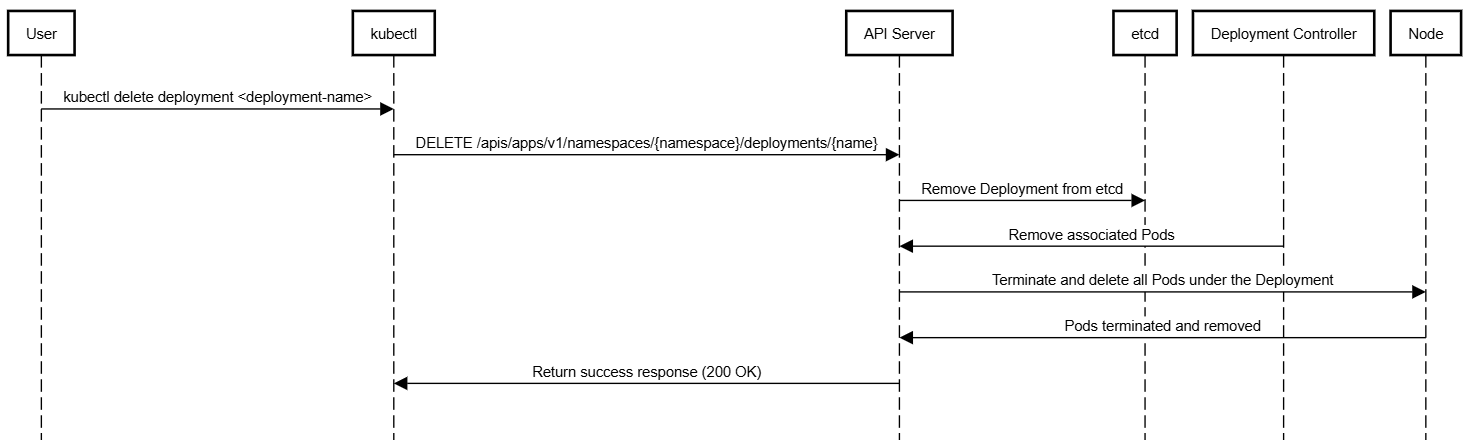
\includegraphics[width=\textwidth]{../uml_seq_diagrams/create_deployment.png}
    \caption{Creating a Deployment}
    \label{fig:create_deployment_diagram}
\end{figure}

During validation, if the YAML file has missing or invalid fields (e.g., no container image specified), or if the user lacks the necessary permissions, the API detects this error, and returns one the following error codes: 
\begin{itemize}
    \item 400 Bad Request: If the YAML syntax or required fields are incorrect.
    \item 403 Forbidden: If the user lacks permissions to create resources in the specified namespace.
    \item 409 Conflict: If a Pod with the same name already exists in the namespace.
\end{itemize}

\begin{figure}[H]
    \centering
    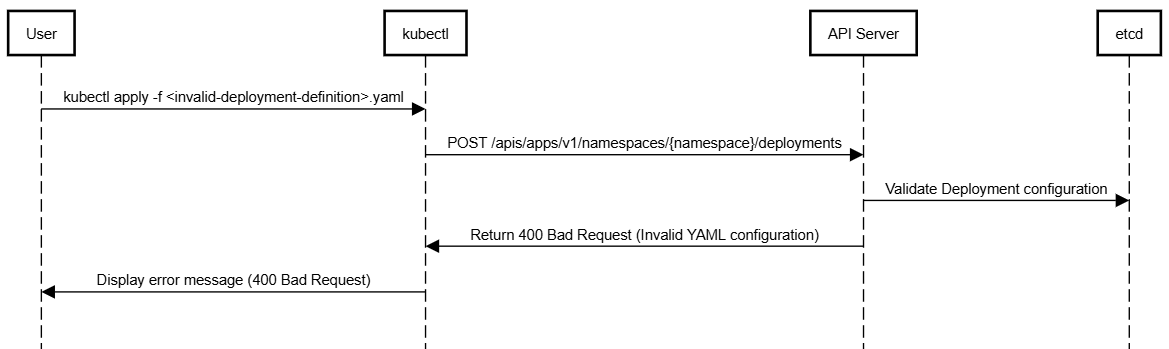
\includegraphics[width=\textwidth]{../uml_seq_diagrams/error_creating.png}
    \caption{Error During Creating a Deployment}
    \label{fig:create_deployment_diagram}
\end{figure}

For the purposes of our testing, we simplify this process by focusing on individual Pod creation rather than a full Deployment. This involves defining a YAML file with metadata and container specifications for the Pod and running \texttt{kubectl apply -f <pod-definition>.yaml}. This request places the Pod in the Pending state as it waits for resources, without the additional management and scaling features provided by a Deployment. The Pod's status can be checked with \texttt{kubectl get pod <pod-name>}.

\paragraph{Note:} From now on, our focus is primarily on the user-level interactions involved in creating and managing Pods, particularly the modifications to their YAML descriptions. While Kubernetes encompasses complex internal interactions, such as scheduling and resource allocation, our analysis centers on the direct commands issued by the user and the resulting states of the Pods. Therefore, UML diagrams will not be provided for every transition tested, as many involve similar user interactions: modifying YAML configurations followed by applying them with \texttt{kubectl apply -f <pod-definition>.yaml}. 

The following figures illustrate the most important user-level interactions, including both positive and negative call flows:
    
\begin{figure}[H]
    \centering
    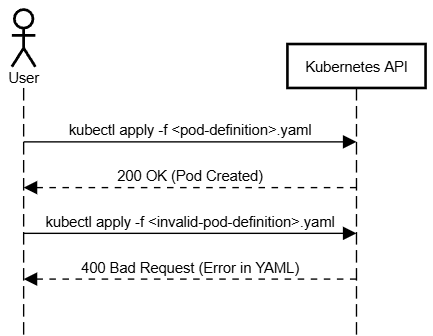
\includegraphics[width=0.5\textwidth]{../uml_seq_diagrams/kubectl_apply.png}
    \caption{Apply pod definition}
    \label{fig:apply_pod_def_diagram}
\end{figure}

\begin{figure}[H]
    \centering
    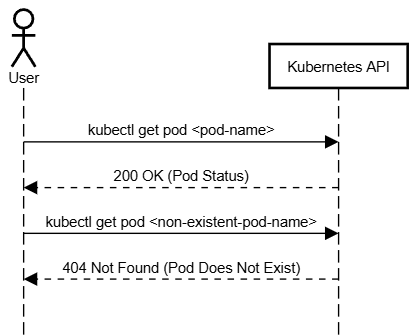
\includegraphics[width=0.5\textwidth]{../uml_seq_diagrams/kubectl_get_pod.png}
    \caption{Get the status of the pod}
    \label{fig:get_pod_diagram}
\end{figure}

\begin{figure}[H]
    \centering
    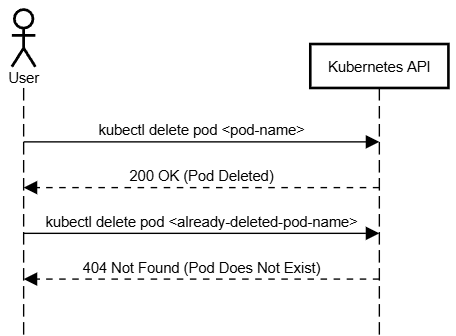
\includegraphics[width=0.5\textwidth]{../uml_seq_diagrams/kubectl_delete.png}
    \caption{Delete a pod}
    \label{fig:delete_pod_diagram}
\end{figure}


\subsubsection{Image Pull Error (Pending $\rightarrow$ ImagePullBackOff)}
If a Pod is unable to pull the specified container image, it transitions to the ImagePullBackOff state. This can happen due to reasons such as the image not existing or the user not having the necessary permissions to access the image registry. To trigger this transition for testing, we can create a Pod with an invalid image name. Upon executing \texttt{kubectl apply -f <pod-definition>.yaml}, the Pod will enter the ImagePullBackOff state, which can be verified by running \texttt{kubectl get pod <pod-name>}. The status will indicate that the Pod is in ImagePullBackOff.

\subsubsection{Image Pull Success (Pending or ImagePullBackOff $\rightarrow$ ContainerCreating)}
When the container image is successfully pulled, the Pod moves from the Pending (or the ImagePullBackOff) state to the ContainerCreating state. During this state, Kubernetes prepares the environment for the container, setting up the network, storage, and any other necessary configurations. This transition can be tested by creating a Pod with a valid image. Upon running \texttt{kubectl apply -f <pod-definition>.yaml} and checking the status with \texttt{kubectl get pod <pod-name>}, the Pod should transition to ContainerCreating.

\subsubsection{Containers Ready (ContainerCreating $\rightarrow$ Running\_NotReady)}
After the environment is set up, the containers within the Pod are started. If they are not yet ready to serve requests, the Pod is in the Running\_NotReady state. To test this, we can deploy a Pod with a readiness probe configured to fail initially. After running \texttt{kubectl apply -f <pod-definition>.yaml} and checking its status, it will show the Pod in Running\_NotReady when we check its status.

\subsubsection{Readiness Probe Success (Running\_NotReady or Running\_Ready $\rightarrow$ Running\_Ready)}
Once the readiness probe passes, the Pod transitions to the Running\_Ready state (or stays in Running\_Ready state), indicating that it is fully operational. This can be tested by modifying the readiness probe of the previous Pod to succeed after a short delay. Once the Pod has started and the readiness probe passes, running \texttt{kubectl get pod <pod-name>} will show the status as Running\_Ready.

\subsubsection{Readiness Probe Failure (Running\_Ready or Running\_NotReady $\rightarrow$ Running\_NotReady)}
If the readiness probe fails, the Pod returns to the Running\_NotReady state (or stays in Running\_NotReady state). This can occur if the application within the container is unable to respond correctly. To test this transition, we can modify the application to simulate a failure in response to the readiness probe. After deploying the Pod with this failing application, the status can be checked with \texttt{kubectl get pod <pod-name>} to confirm the transition.

\subsubsection{Pod Success (Running\_Ready $\rightarrow$ Succeeded)}
When a Pod completes its task successfully and all containers exit without errors, it moves to the Succeeded state. This is used for batch jobs rather than for average pods. We can test this by creating a job-type pod that runs a command that exits with a zero status. After deploying the Pod, checking its status with \texttt{kubectl get pod <pod-name>} will show that it has moved to the Succeeded state.

\subsubsection{Pod Failure (Running\_Ready $\rightarrow$ Failed)}
If a container within a Pod exits with a non-zero status, indicating an error, the Pod transitions to the Failed state. We can test this by deploying a Pod that is designed to fail during execution. After the Pod runs, checking its status with \texttt{kubectl get pod <pod-name>} will show that it has moved to the Failed state.

\subsubsection{Container Crash Loop (Running\_NotReady $\rightarrow$ CrashLoopBackOff)}
When a container in a Pod fails repeatedly during startup, the Pod enters the CrashLoopBackOff state. This transition indicates that the system is trying to restart the container but is unable to do so successfully. To test this, we can deploy a Pod with a configuration that intentionally causes the container to fail on startup. Observing the Pod’s status with \texttt{kubectl get pod <pod-name>} will reveal the transition to CrashLoopBackOff.

\subsubsection{Crash Loop Timeout (CrashLoopBackOff $\rightarrow$ Running\_NotReady)}
If a Pod remains in the CrashLoopBackOff state for too long without a successful start, it will transition back to the Running\_NotReady state. This indicates that the system is no longer attempting to restart the container. To test this transition, we can simulate a prolonged crash loop and wait for the timeout. After the timeout, checking the Pod’s status will confirm its return to Running\_NotReady.

\subsubsection{Delete Pod (All States $\rightarrow$ Terminating)}
Issuing a delete command for a Pod in any state causes it to transition to the Terminating state. This transition ensures that the Pod is in the process of being removed from the cluster. To test this, we can run the command \texttt{kubectl delete pod <pod-name>} and then check the Pod’s status. It should show that it is in the Terminating state.

\subsubsection{Final Deletion (Terminating $\rightarrow$ PodNotExists)}
Once a Pod has been marked for termination, Kubernetes performs automatic cleanup processes. After these processes are complete, the Pod no longer exists in the cluster. To verify this transition, we can issue the delete command using \texttt{kubectl delete pod <pod-name>} and then attempt to check the status with \texttt{kubectl get pod <pod-name>}. If the Pod has been successfully removed, we will receive an error indicating that the Pod no longer exists, confirming the transition from Terminating to a non-existent state.



\end{document}